\documentclass{beamer}
%\mode<presentation> {

\usetheme{Berlin}
%\usecolortheme{beaver}
\usepackage{graphicx}
\usepackage{booktabs}
\setbeamertemplate{footline}[page number]
\setbeamertemplate{navigation symbols}{}
\setkeys{Gin}{width=0.35\textwidth}
\title[CLM 2015]{Cumulative Link Models}
\author{Josh Lospinoso, PhD}

\institute{
\textit{josh@lospi.net}
}
\date{\today}

\usepackage{Sweave}
\begin{document}
\input{presentation-concordance}

\begin{frame}
\titlepage
\end{frame}

\begin{frame}
\frametitle{Overview}
\tableofcontents
\end{frame}


\section{Statistical Modeling}
\begin{frame}
Let's start with some philosophy (on statistical modeling...)
\end{frame}

\begin{frame}
\begin{figure}
\centering
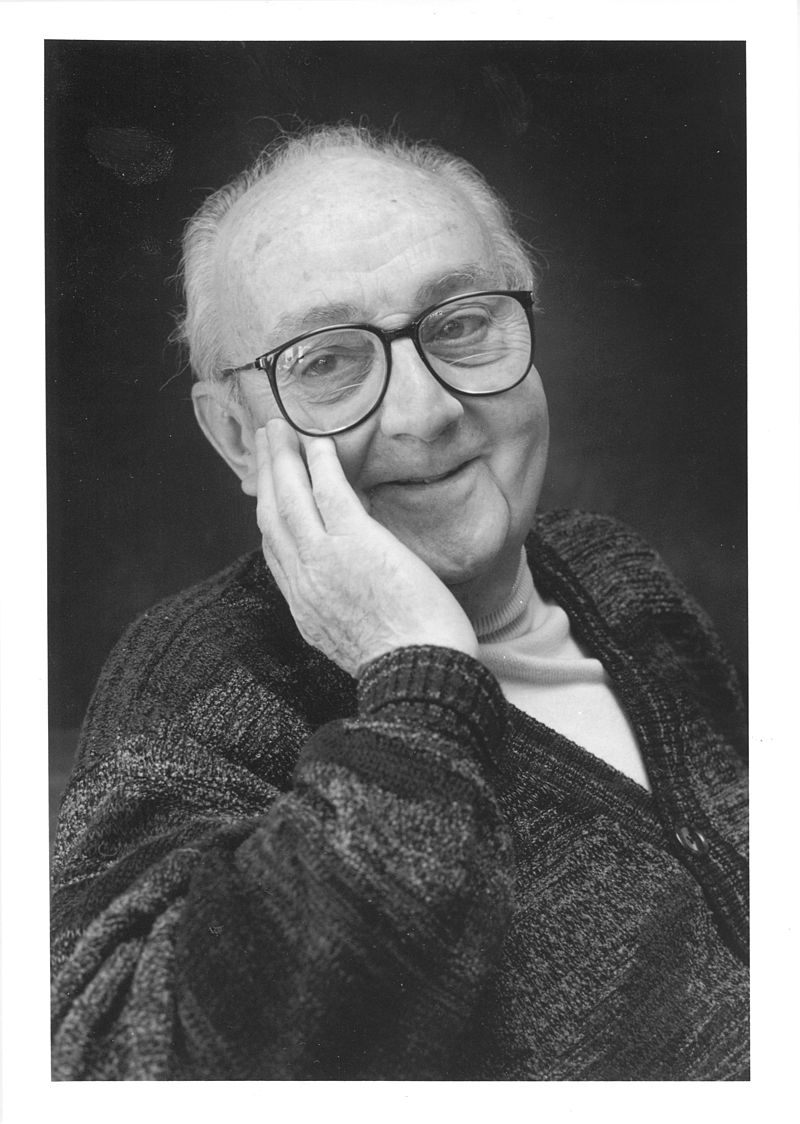
\includegraphics[width=.3\textwidth]{800px-GeorgeEPBox}
\label{fig:george_box}
\end{figure}
\begin{center}
\textbf{"All models are wrong but some are useful."} 

\vspace{10px}

George E.P.\ Box (1978)
\end{center}
\end{frame}




\begin{frame}{Linear Regression}
\begin{figure}
\centering
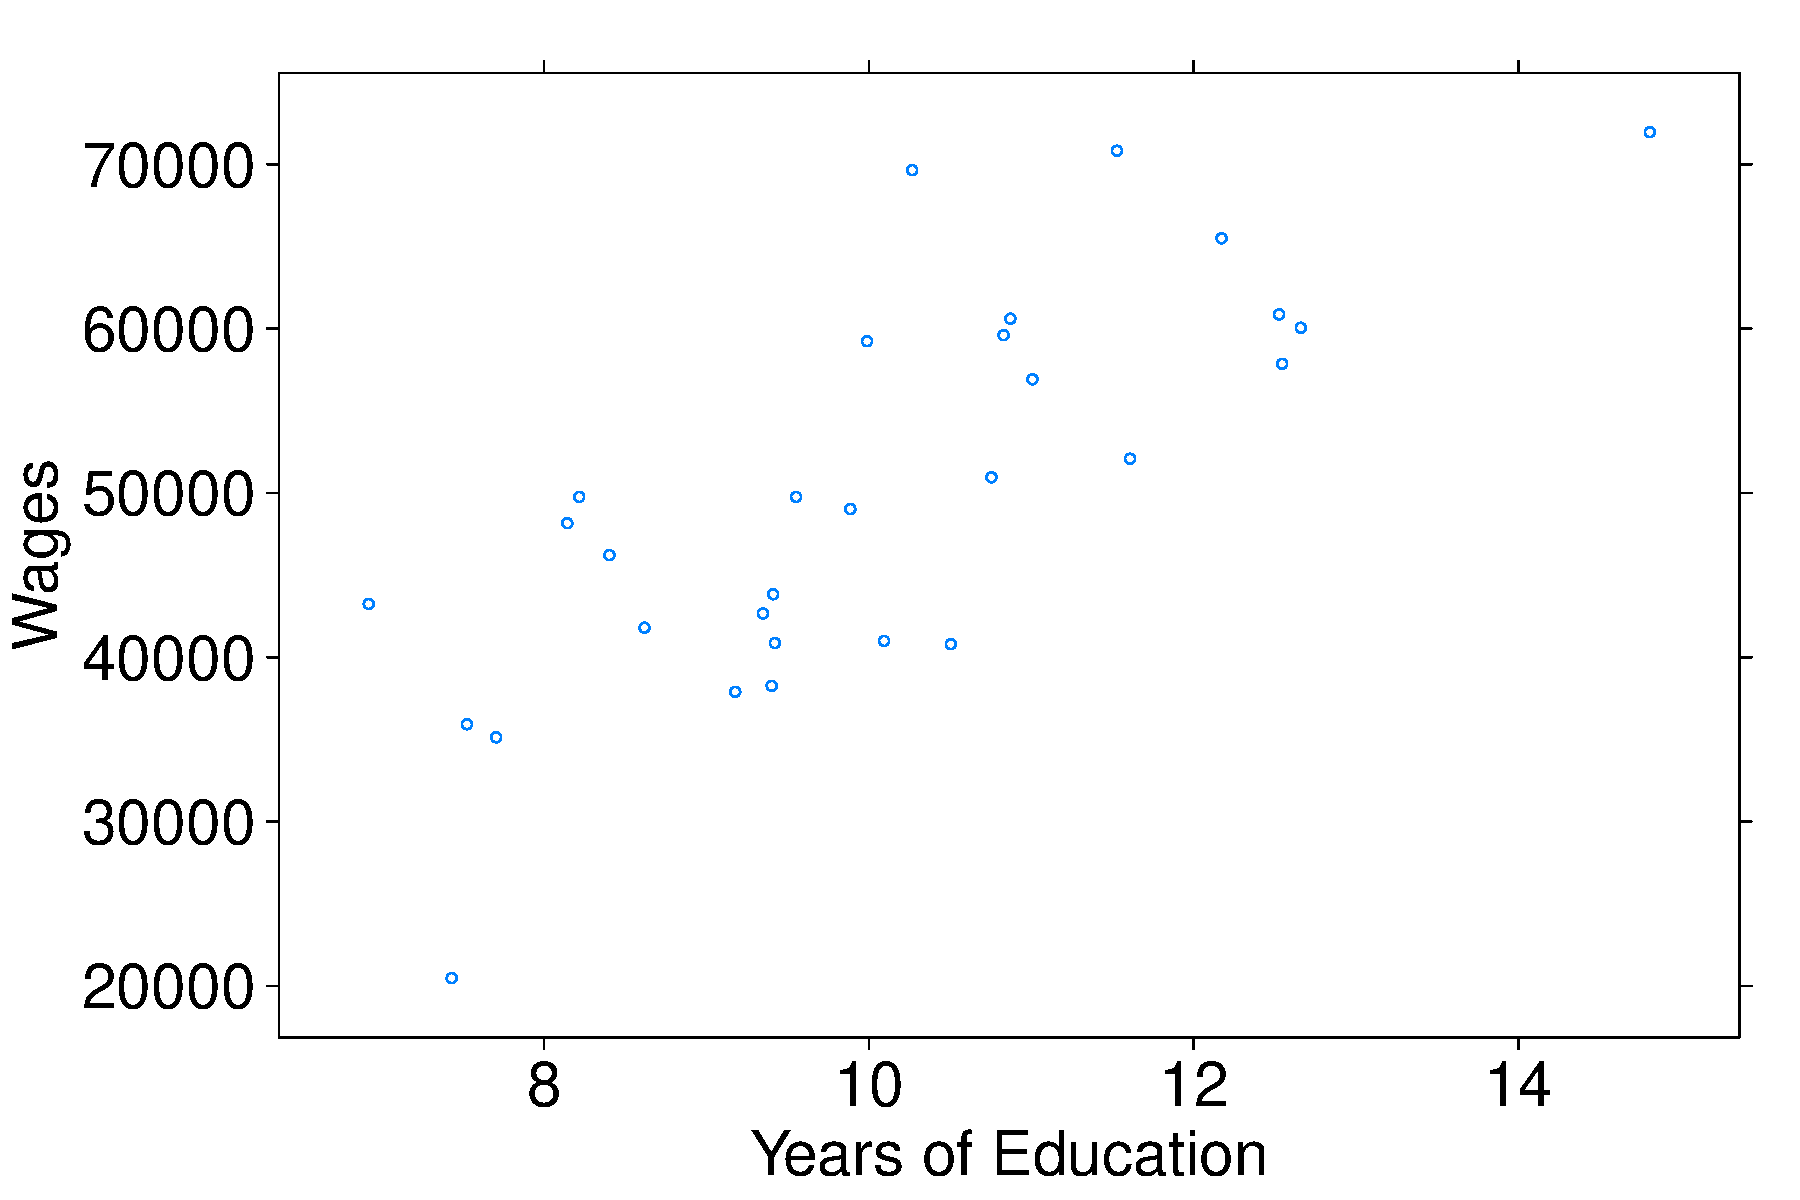
\includegraphics[width=0.8\textwidth]{linreg_plot_1}
\label{fig:linreg_plot_1}
\end{figure}
\end{frame}

\begin{frame}{Linear Regression}
\begin{figure}
\centering
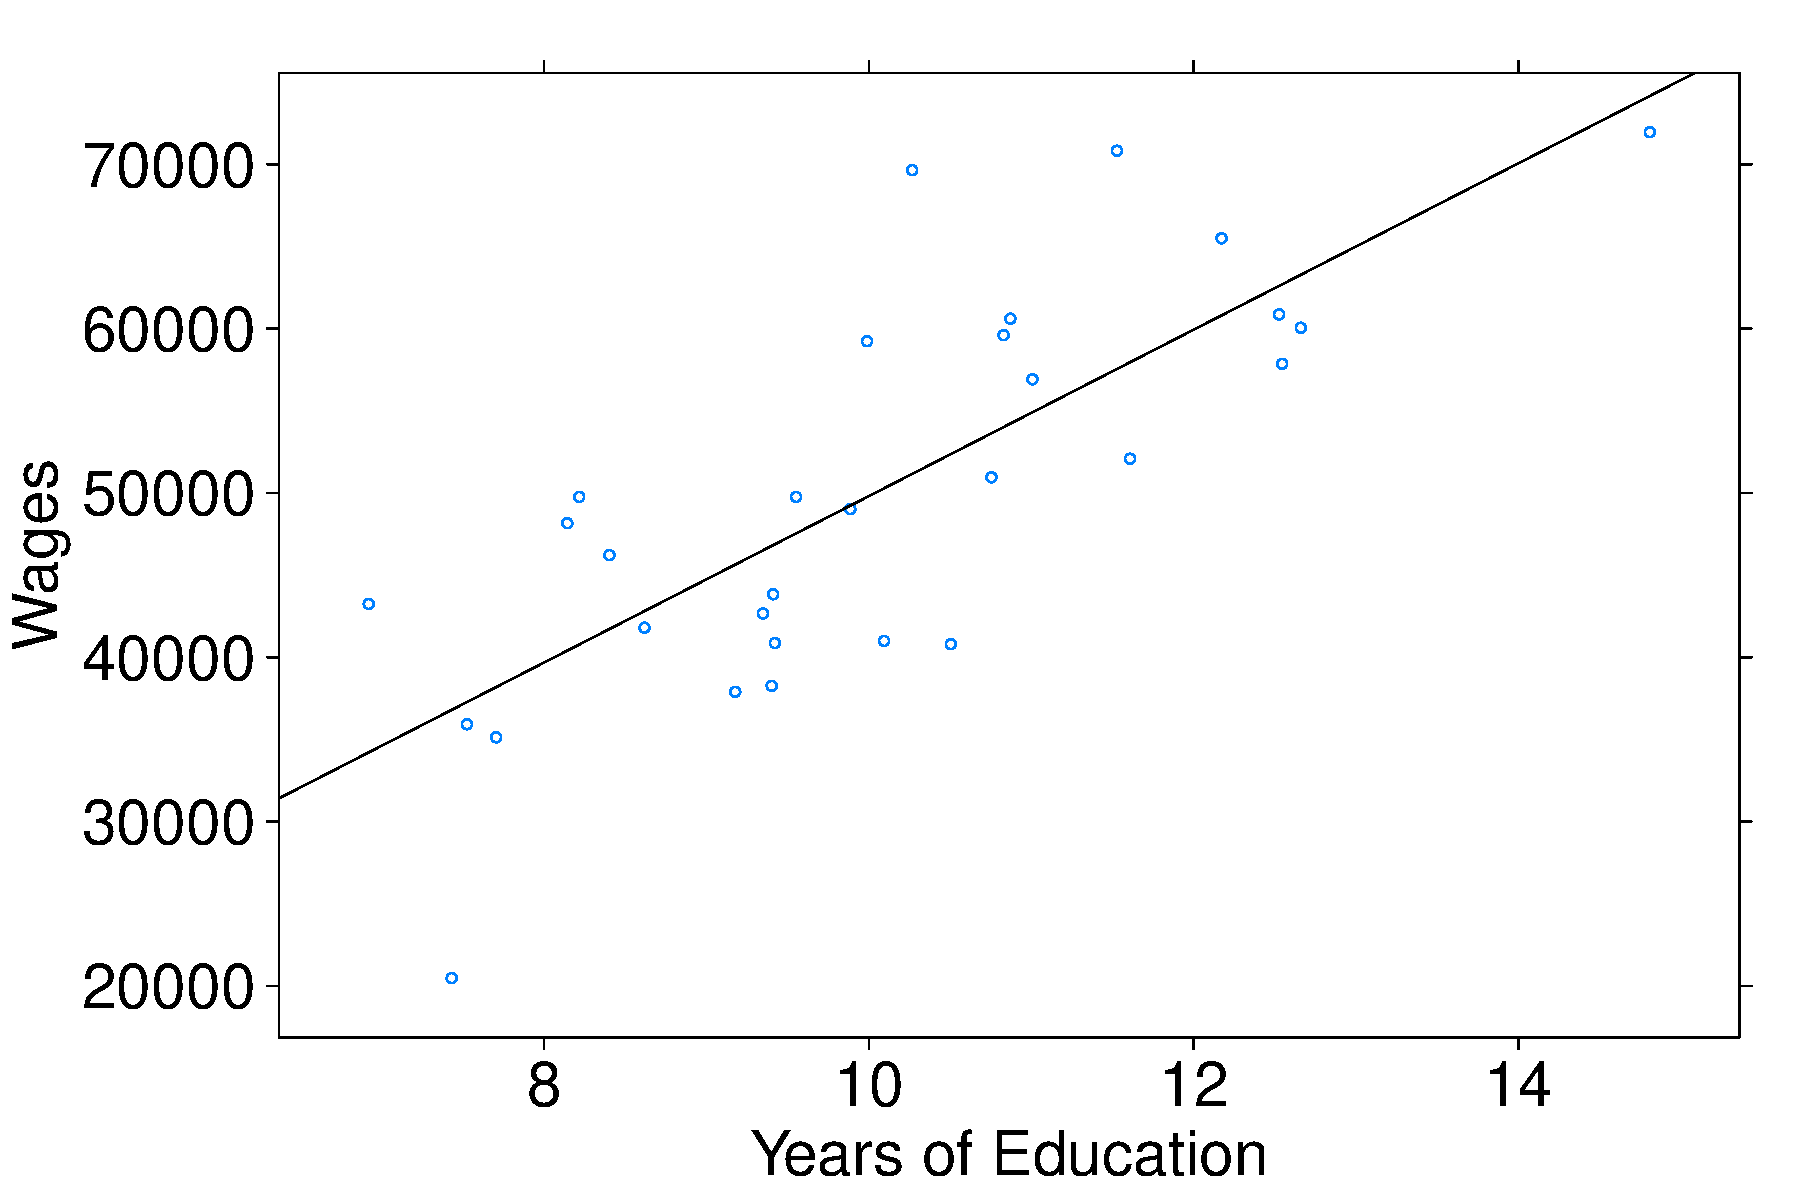
\includegraphics[width=0.8\textwidth]{linreg_plot_2}
\label{fig:linreg_plot_2}
\end{figure}

Slope $\approx$ 5000 dollars per year (and, importantly, we can get p-values...)
\end{frame}

\begin{frame}
Such models are certainly not how reality works.

\vspace{20px}

But they can \emph{illuminate} some phenomena we care about.

\vspace{20px}

Researchers in many disciplines have been taking this approach for decades. It works (and, importantly, scholarly journals tend to recognize this kind of analysis!)
\end{frame}

\begin{frame}{Parametric and Non-parametric Statistics}
Consider these hypotheses (taken from Stuart et.\ al.\ 1999):
\begin{enumerate}
\item that a normal distribution has a specified mean and variance
\item it has a given mean but unspecified variance
\item a distribution is of normal form with both mean and variance unspecified
\item that two unspecified continuous distributions are identical
\end{enumerate}
\vspace{10px}
1/2 are \emph{parametric} hypotheses, 3/4 are \emph{non-parametric}.
\end{frame}

\section{Ordinal Categorical Data}
\begin{frame}{Continuous Data}
\begin{itemize}
\item Speed
\item Weight
\item Distance
\item Time
\end{itemize}
Continuous data \emph{not countable}.
\end{frame}

\begin{frame}{Discrete Data}
\begin{itemize}
\item Die roll
\item Number of patients
\item MCAT score
\end{itemize}
\vspace{10px}
Discrete data is \emph{countable}.
\end{frame}

\begin{frame}{Categorical Data}
\begin{itemize}
\item Gender
\item Race
\item Hair color
\end{itemize}
Categorical data is about \emph{group membership}.
\end{frame}

\begin{frame}{Ordinal Categorical Data}
\begin{itemize}
\item Stages of illness (e.g.\ stage 3 cancer)
\item Questionnaires (e.g.\ ``In general, how is your health?'')
\item Modified Fitzpatrick scale (i.e.\ complexion)
\end{itemize}
Categorical data is about \emph{ordered group membership}.
\end{frame}

\begin{frame}{Ordinal Categorical Data}
In this talk, we focus on a kind of data that is common when studying pathologies.

\vspace{20px}

\textbf{Ordinal}, \textbf{categorical} data exists on an \textbf{arbitrary numerical scale}. The exact numerical quantity \textbf{has no significance beyond its ability to establish ranking}.

\vspace{20px}

I hope to convince you that this kind of data needs \textbf{special treatment}! (Linear models and ANOVAs simply won't do.)
\end{frame}

\section{Cumulative Link Model}
\begin{frame}{Cumulative Link Model}
CLMs are well suited to ordinal, categorical data. They:

\begin{enumerate}
\item provide a flexible regression framework to answer nuanced questions,
\item allow you to wring every ounce of power out of your data, and
\item can protect you from some kinds of inferential errors.
\end{enumerate}

If you have this kind of data, CLMs are your go-to tool!
\end{frame}

\begin{frame}{A Running Example}
\begin{figure}
\centering
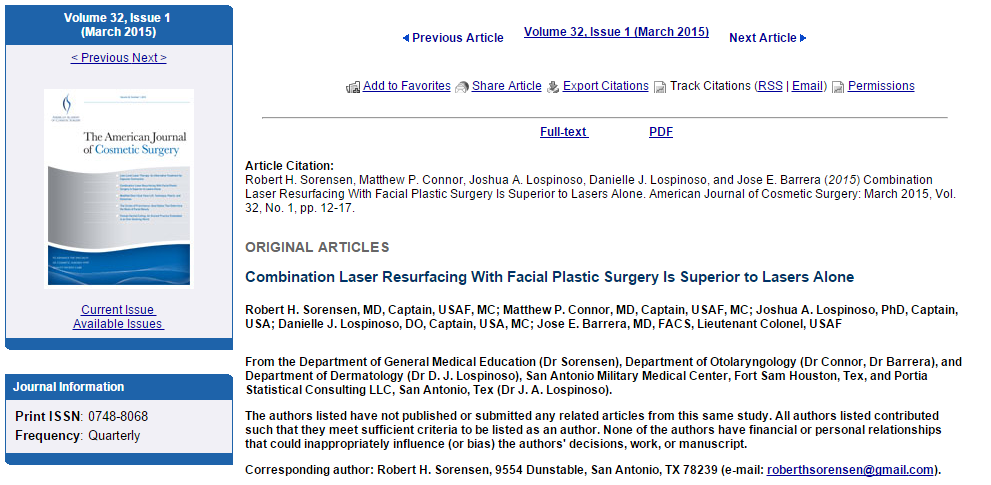
\includegraphics[width=1.1\textwidth]{Sorensen2015}
\label{fig:sorensen_2015}
\end{figure}
\end{frame}

\begin{frame}
\textbf{Hypothesis}: When treating rhytidosis, combining facial plastic surgery with CO$_2$ fractional laser treatment is superior to laser treatment alone.

\vspace{25pt}

Two pathologists evaluate Modified Fitzpatrick and Glogau before and after treatment
\end{frame}

\begin{frame}
For each observation in Sorensen (2015), we have:

\begin{itemize}
\item Glogau after procedure(s)
\item Modified Fitzpatrick after procedure(s)
\item Laser?
\item Pathologist ID
\item Patient ID
\item Estimated Age
\item Modified Fitzpatrick before procedure(s)
\item Glogau before procedure(s)
\end{itemize}
\end{frame}

\begin{frame}{Textual Presentation}
There is some non-zero probability that a pathologist rates a patient each of the possible Glogau/Modified Fitzpatrick levels.

\vspace{10px}

Each explanatory term (e.g.\ laser, estimated age, and Glogau before procedures) can have a profound effect on these probabilities.

\vspace{10px}

\textbf{We want to infer about these effects!}
\end{frame}

\begin{frame}{Technical Presentation}
Ordinal response variables $Y_i$ falls in category $j$ with probability $\pi_{ij}$.

\vspace{10px}

Cumulative probabilities are therefore:
\begin{equation}
\gamma_{ij}=P(Y_i \leq j) = \pi_{i1}+...+\pi{ij}
\end{equation}

\vspace{10px}

The CLM is a regression of \emph{cumulative logits}
\begin{equation}
\mbox{logit}(\gamma_{ij}) = \theta_j + x_i^T\beta
\end{equation}
where 
\begin{itemize}
\item $x$ are the explanatory terms
\item $\beta$ is the \emph{effect} parameter
\item $\theta_j$ is a constant for category $j$
\end{itemize}
\end{frame}


\begin{frame}{Graphical Presentation}
\begin{figure}
\centering
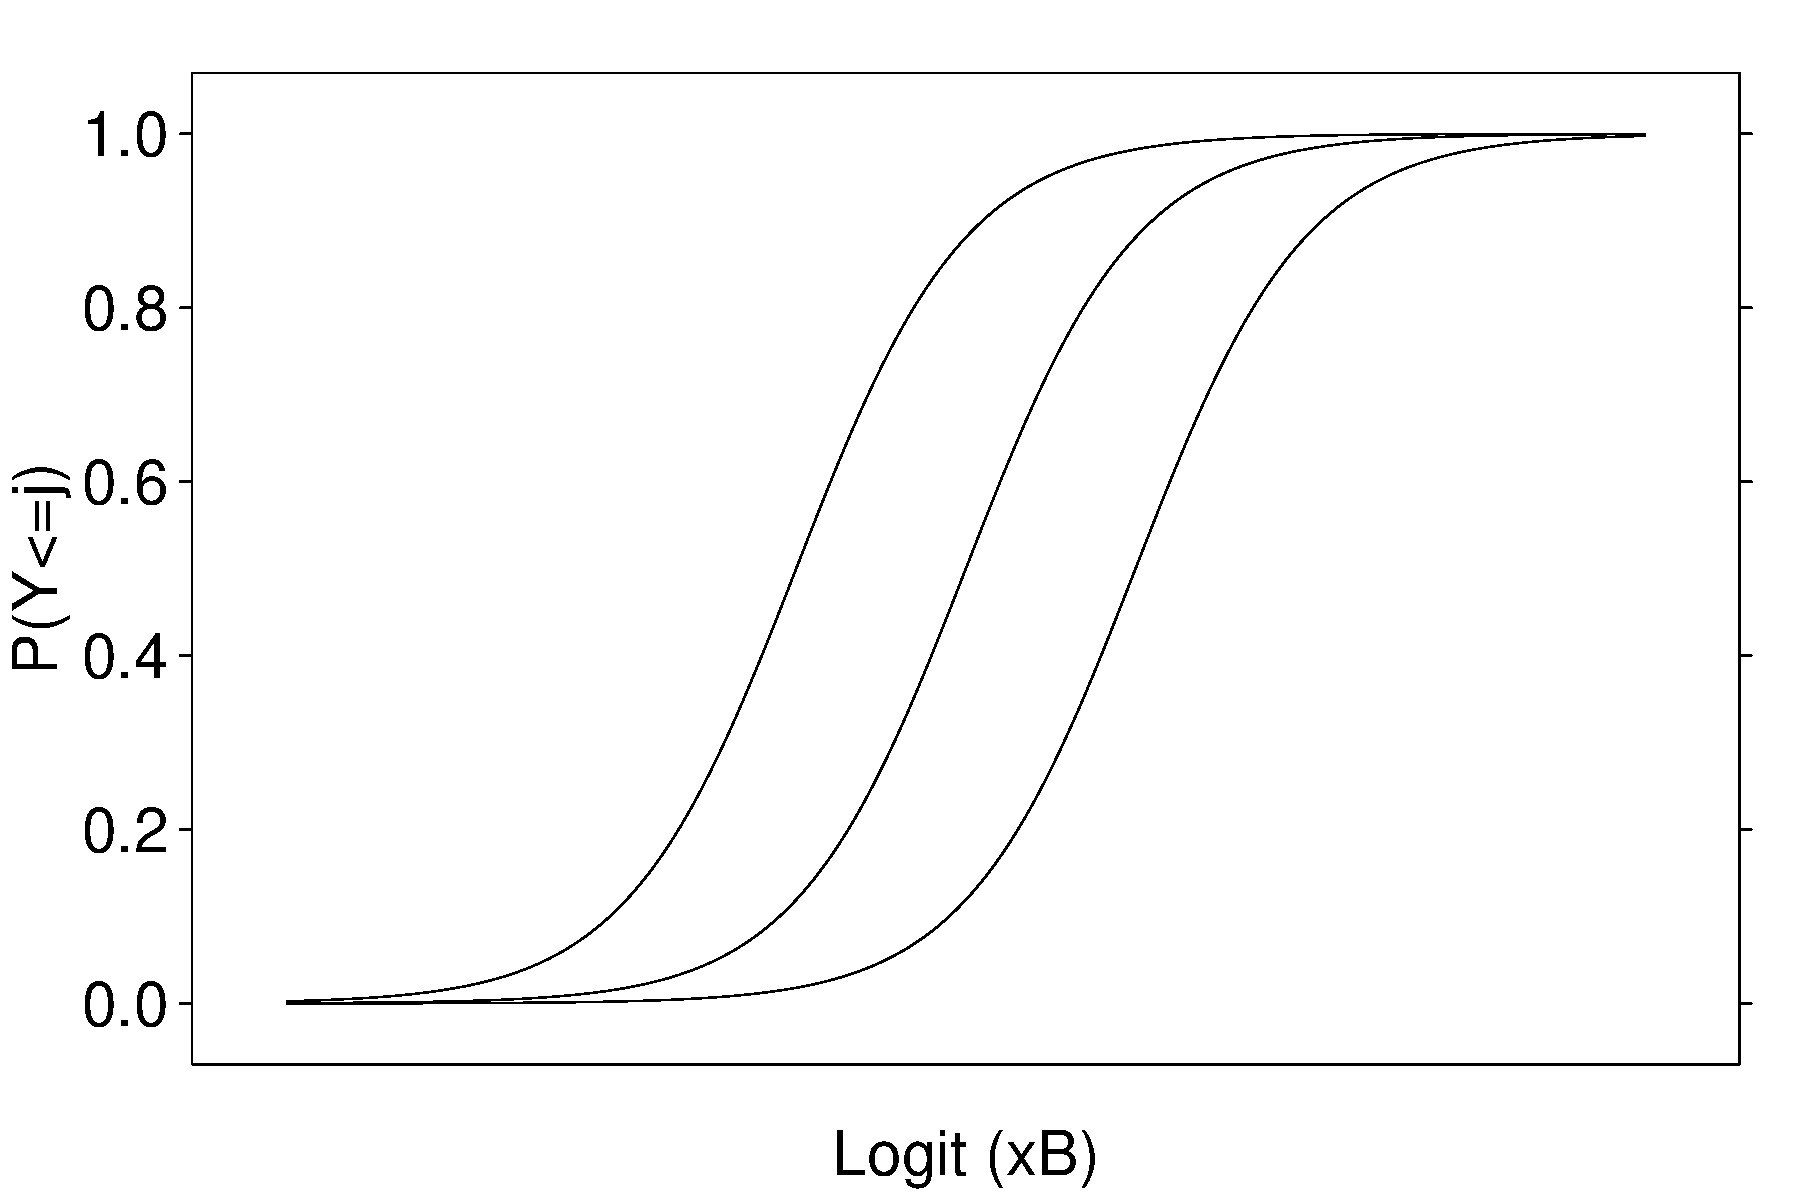
\includegraphics[width=0.8\textwidth]{clm_plot}
\label{fig:clm_plot}
\end{figure}
\end{frame}

\section{What Could Go Wrong?}
\begin{frame}{What Could Go Wrong?}
Consider a fictitious dataset generated by a CLM:
\begin{itemize}
\item 100 observations
\item Response $Y$ on a scale from 1 to 5
\item Two explanatory terms: $X_1$ and $X_2$
\item $Y$ depends on $X_2$, but not on $X_1$
\end{itemize}
\end{frame}


\begin{frame}
Using this setup, we generate hundreds of thousands of sample datasets, e.g.:

\begin{figure}
\centering
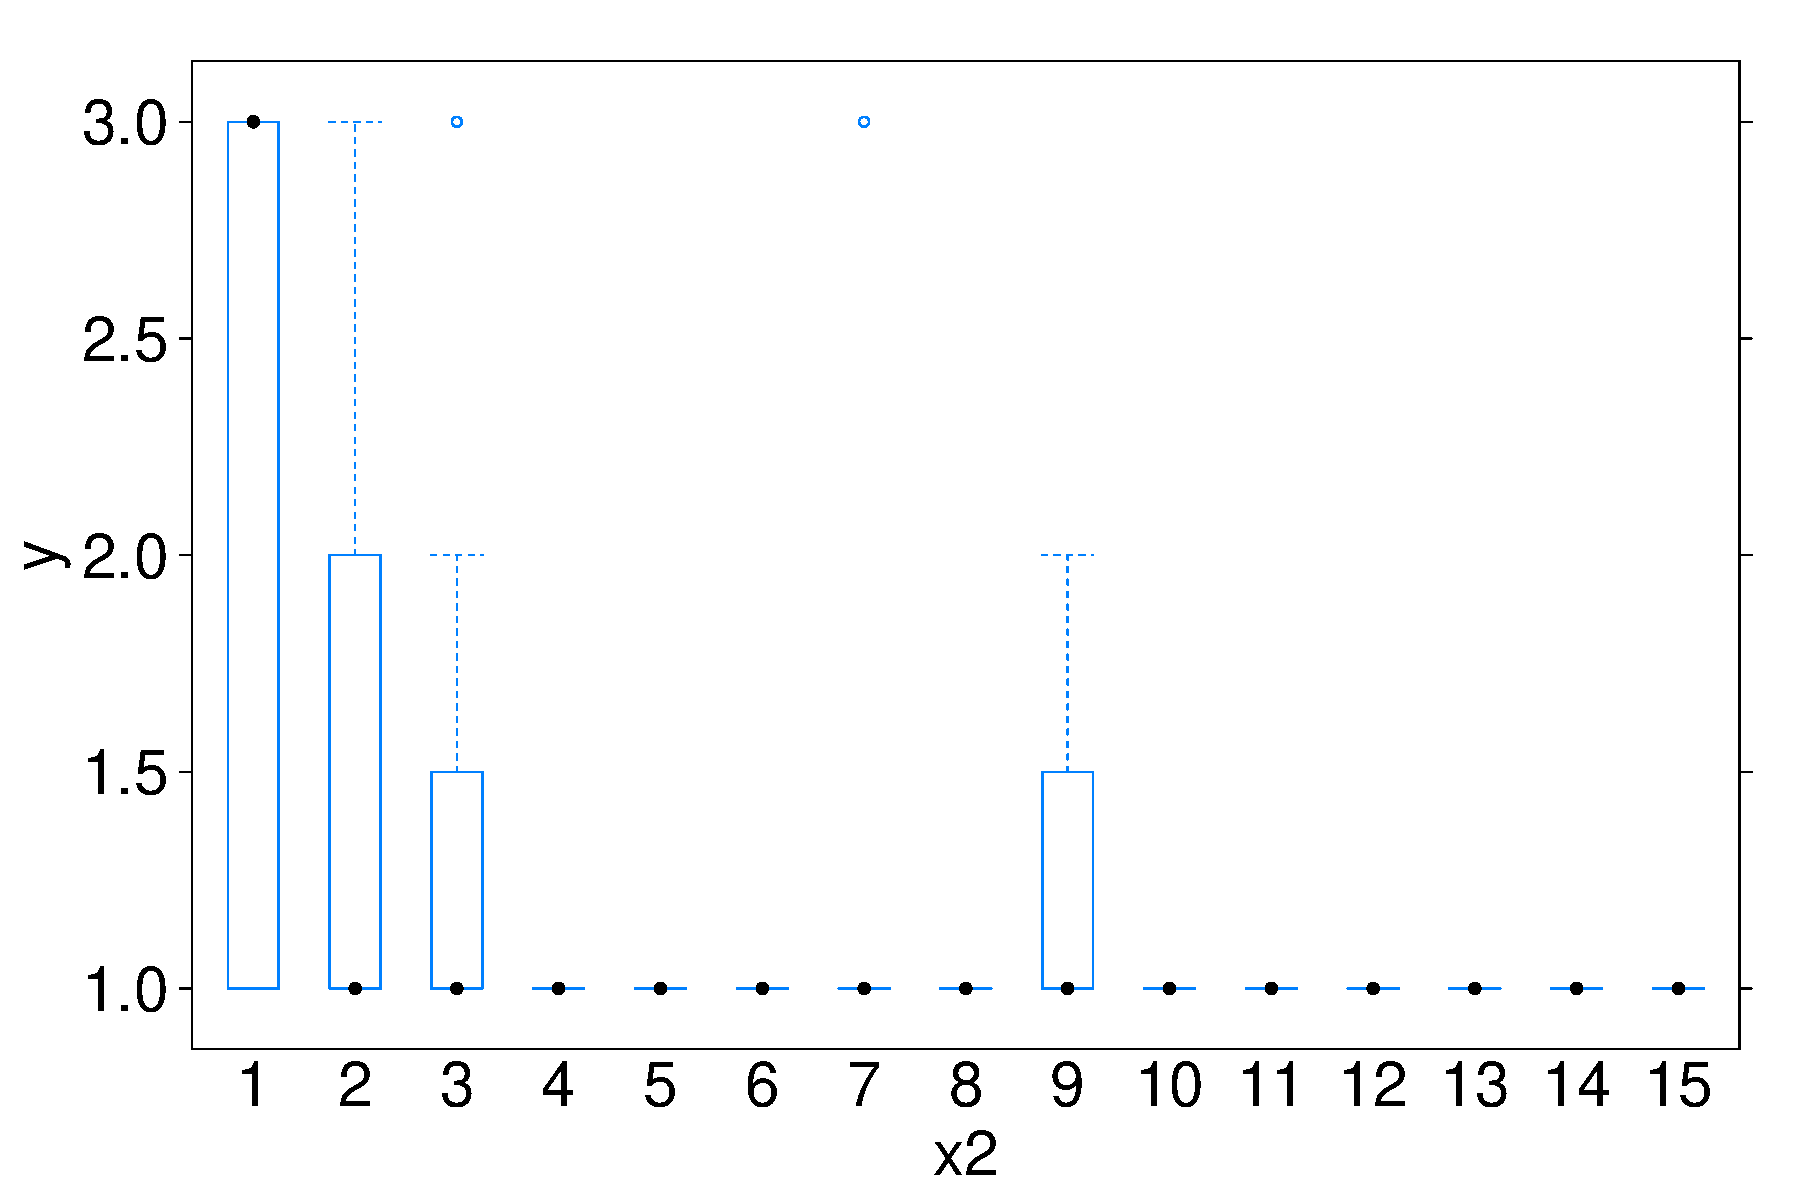
\includegraphics[width=.9\textwidth]{sample_boxplot}
\caption{Sample dataset generated by CLM.}
\label{fig:sample_boxplot}
\end{figure}
\end{frame}

\begin{frame}[fragile]
We can estimate the parameters easily using the R package \texttt{ordinal}:
\begin{block}{Estimating with \texttt{ordinal}}
\begin{Schunk}
\begin{Sinput}
> my.model <- clm(y~x1+x2, data=sample.data)
> confint(my.model)
\end{Sinput}
\begin{Soutput}
       2.5 %      97.5 %
x1 -1.316768 -0.05512462
x2 -0.676549  0.42723845
\end{Soutput}
\end{Schunk}
\end{block}

\emph{The generative model has $X_1$'s parameter at $-0.5$}
\end{frame}

\begin{frame}
One (unfortunately) typical approach to ordinal data is to use a Gaussian linear
model, e.g.\ nested in an ANOVA approach.

\begin{itemize}
\item What happens if we use a \emph{linear model} to estimate CLM data?
\item How much \emph{power} do we lose?
\item Are our \emph{false positives} inflated?
\end{itemize}
\end{frame}


\begin{frame}
\begin{figure}
\centering
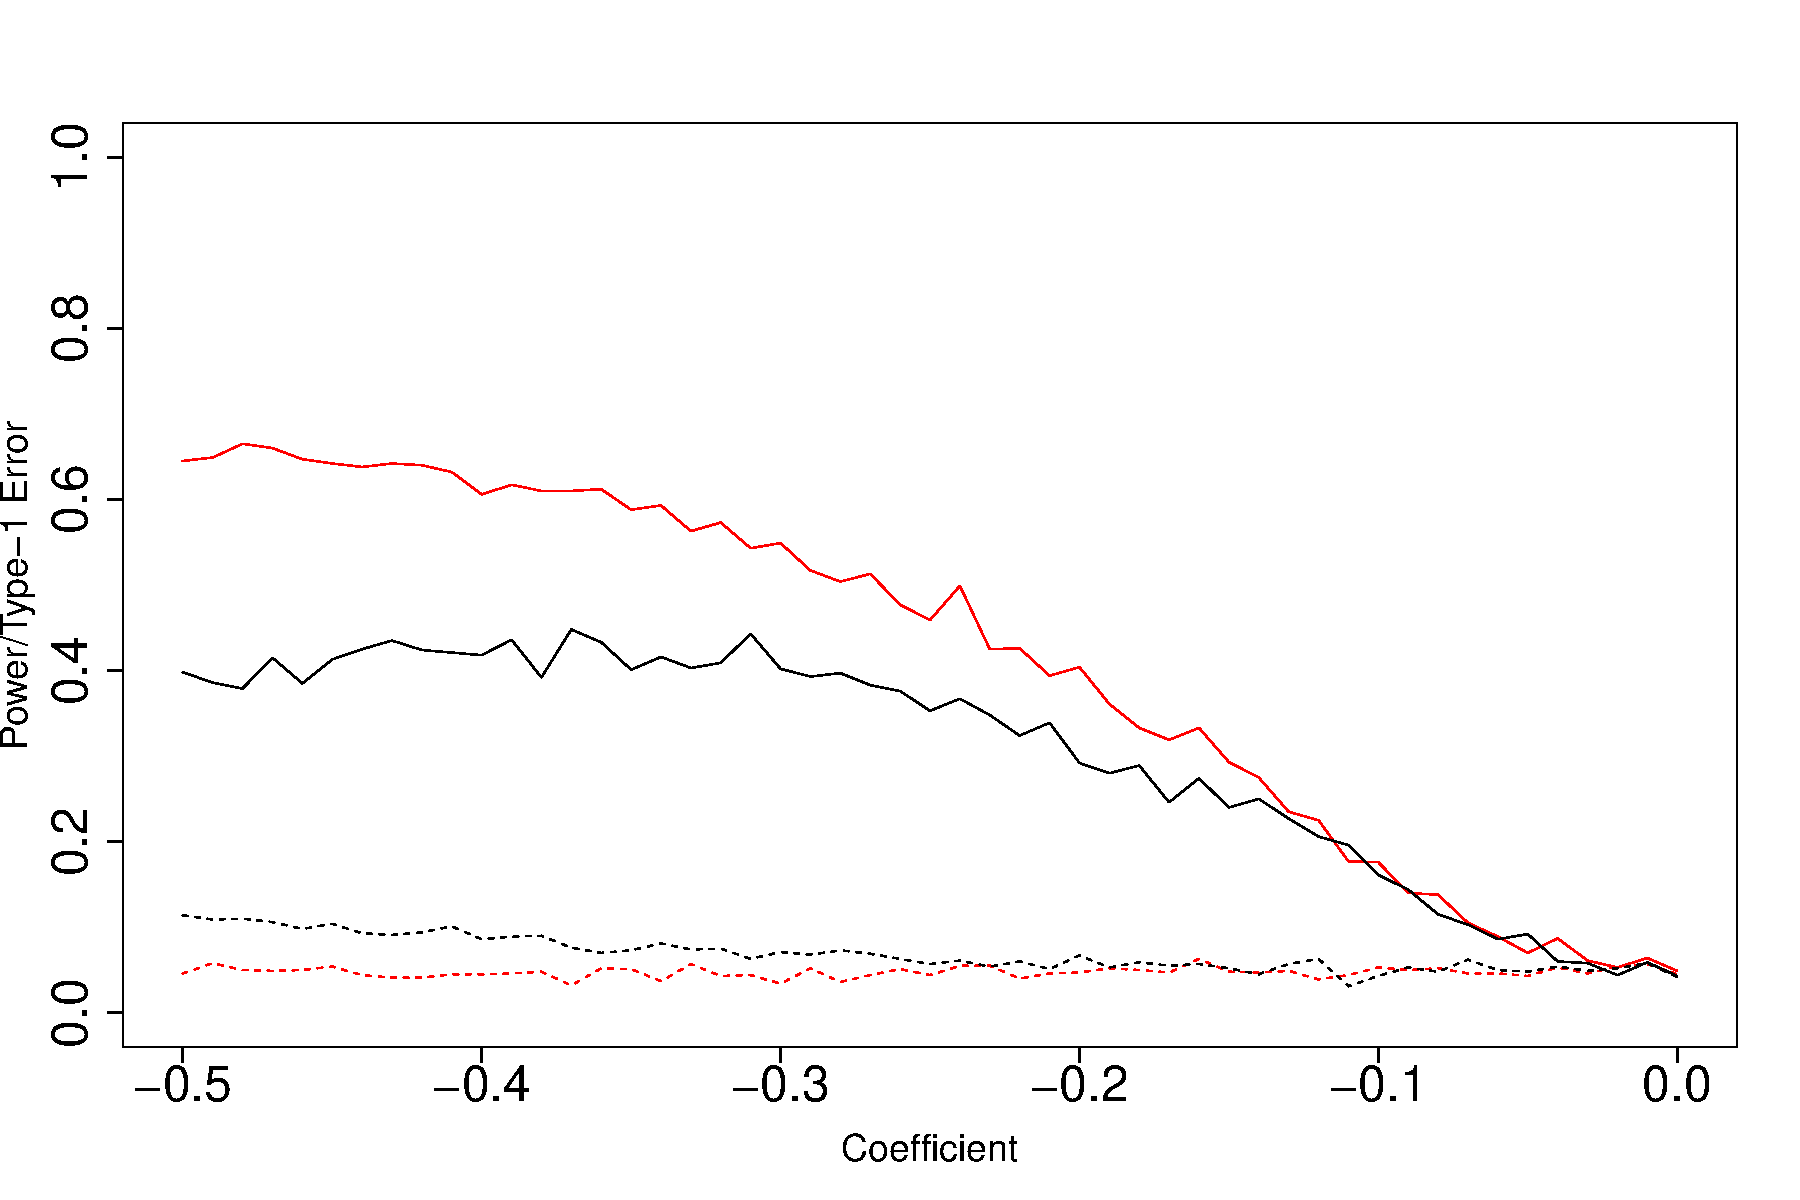
\includegraphics[width=1.0\textwidth]{experiment_plot}
\caption{Red: CLM t-test. Black: LM t-test. Solid: X1. Dotted: X2.}
\label{fig:sample_boxplot}
\end{figure}
\end{frame}

\begin{frame}
Some other (more technical) reasons not to use a linear model (see Christensen 2015):

\begin{itemize}
\item \emph{standard errors are inappropriate}: residuals cannot be normally distributed
\item \emph{inflation of information in the data}: linear models assume a scale between categories
\end{itemize}
\end{frame}

\section{Example}
\begin{frame}{Example}
\begin{figure}
\centering
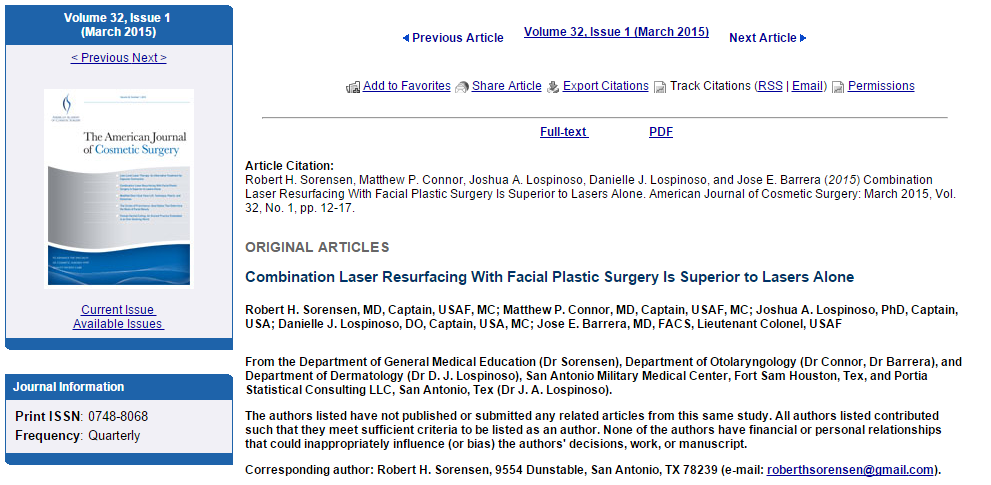
\includegraphics[width=1.1\textwidth]{Sorensen2015}
\label{fig:sorensen_2015}
\end{figure}
\end{frame}

\begin{frame}
\textbf{Hypothesis}: When treating rhytidosis, combining facial plastic surgery with CO$_2$ fractional laser treatment is superior to laser treatment alone.

\vspace{25pt}

Two pathologists evaluate Modified Fitzpatrick and Glogau before and after treatment
\end{frame}

\begin{frame}
  \begin{table}[]
  \centering
  \caption{Golgau via CLM estimation (probit)}
  \label{my-label}
  \begin{tabular}{lrr} \hline
            & Estimate & p-value \\ \hline \hline
  Treatment & -0.78    & 0.07    \\
  Rater     & -0.18    & 0.61    \\
  Est. Age  &  0.10    & 0.00    \\
  Fitz. 345 & -1.42    & 0.00    \\
  Glogau 34 &  1.61    & 0.02    \\ \hline
  \end{tabular}
  \end{table}
\end{frame}

\begin{frame}
  \begin{table}[]
  \centering
  \caption{Modified Fitzpatrick via CLM estimation (probit)}
  \label{my-label}
  \begin{tabular}{lrr} \hline
            & Estimate & p-value \\ \hline \hline
  Treatment & -0.06    & 0.83    \\
  Rater     & -1.29    & 0.00    \\
  Est. Age  &  0.06    & 0.00    \\
  Fitz. 345 & -0.54    & 0.09    \\
  Glogau 34 &  0.15    & 0.71    \\ \hline
  \end{tabular}
  \end{table}
\end{frame}

\section{Questions}
\begin{frame}
\frametitle{References}
  \footnotesize{
  \begin{thebibliography}{99}
  \bibitem[McCullagh, 1989]{p1} P. McCullagh and J. Nelder (1989)
  \newblock Generalized Linear Models, \emph{Chapman and Hall}, Second Ed.
  \bibitem[Sorensen, 2015]{p2} Sorensen, Robert H., et al. (2015)
  \newblock ``Combination Laser Resurfacing With Facial Plastic Surgery Is Superior to Lasers Alone.'' American Journal of Cosmetic Surgery 32.1 (2015): 12-17.
  \bibitem[Christensen, 2015]{p3} Christensen, R. H. B. (2015)
  \newblock ordinal---Regression Models for Ordinal Data. R package version 2015.6-28.
      http://www.cran.r-project.org/package=ordinal/
  \bibitem[]{p4}Stuart A., Ord J.K, Arnold S. (1999)
  \newblock Kendall's Advanced Theory of Statistics: Volume 2A---Classical Inference and the Linear Model, sixth edition.
  \end{thebibliography}
  }
\end{frame}
\begin{frame}
\Huge{\centerline{Questions}}
\end{frame}

\end{document}
%}
